%!TEX root = ../../Main.tex
\graphicspath{{Chapters/System/}}
%-------------------------------------------------------------------------------


\section{System beskrivelse}

BA-TA's (Bluetooth Anti-Theft Alarm) primære funktionalitet ligger i hhv. at kunne låse op og låse hoveddøren, så snart systemet registrerer at husets ejer, og dermed ejerens smartphone, er i nærheden eller ej.

Hele systemet styres fra en samlet enhed, som kan integeres fra brugeren gennem en skærm og dertilhørende touch funktion. 

Igennem brugergrænsefladen kan brugeren både tilføje og fjerne de godkendte Bluetooth-enheder (personer) som skal kunne låse og låse op for døren.

Når alle godkendte enheder er uden for rækkevidde af systemets Bluetooth-modul, låses døren, og så snart systemet ser en godkendt enhed indenfor rækkevidden bliver døren låst op. 

I under-afsnittende herunder bliver systemets blokke og de interne fobindelser præsenteret. Derudover dannes der et overblik over funktionaliteten som er implementeret i projektet og systemet. 
På figur \ref{fig:Bdd} ses et overordnet Bdd for projektet, hvor de interne forbindelser forklares på figur \ref{fig:Ibd}. 

\begin{figure}[H]
	\centering
	\includegraphics[width = 500 pt]{Img/Bdd.png}
	\caption{Bdd af BA-TA}
	\label{fig:Bdd}
\end{figure}

\textbf{***Skal vi nøjes med et mere simpelt BDD hvor der eksempelvis ikke står noger til Arduinoen og de andre?}

\subsection{Blokbeskrivelse BA-TA}
I det følgende vil komme en beskrivelse af de enkelte blokke i BA-TA og deres interne funktionalitet.
\newline
\newline
\textbf{Arduino} \\*
Arduino'en, mega2560, initialiserer og styrer alt funktionaliteten som indgår i systemet. Arduino blokken står for at initialisere  Touch Display, Touch Controller og Display Controller, som bruges til at kunne modtage signaler fra Touch-delen, samt at sende signaler til Display'et og dermed få repræsenteret noget til brugeren. Yderligere bruges Arduinoen til at kommunikkere med Bluetooth-blokken.
\newline
\newline
\textbf{Touch Controller} \\*
Touch Controller står for at modtage værdier fra Touch Display, samt at sende den modtagede værdi videre til Arduino'en. 
\newline
\newline
\textbf{Display Controller} \\*
Display Controller modtager værdier fra Arduino'en og sende sende værdien videre til Touch Display. \newline
\newline
\textbf{Bluetooth} \\*
Bluetooth modul, HC-05, som kommunikkerer med Arduino'en vha. AT-kommandoer.
\newline
\newline
\textbf{Touch Display} \\*
Touch Display fungerer som brugergrænseflade og er dermed måden brugeren kan interagere med systemet. 
\newline
\newline
\textbf{Lock} \\*
Lock er den fysiske lås, denne er ikke implementeret i projektet, men simuleres med en visuel lås på skærmen. 
\subsection{Internal Block Diagram for BA-TA}
På figur \ref{fig:Ibd} ses et overordnet IBD over selve systemet, som er bygget på Bdd'et. 
\begin{figure}[H]
	\centering
	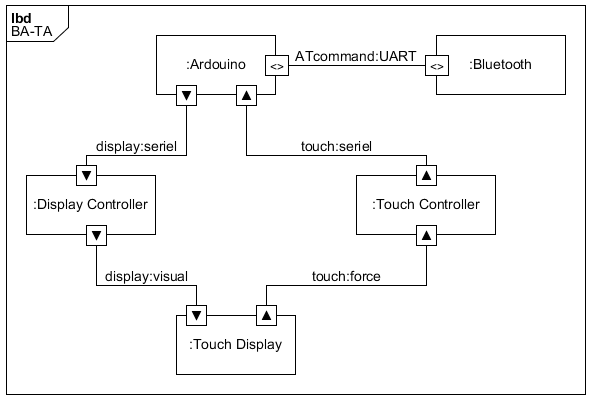
\includegraphics[width = 300 pt]{Img/Ibd.png}
	\caption{Ibd af BA-TA}
	\label{fig:Ibd}
\end{figure}



